\paragraph{}Table 1 bellow shows the measurements taken from the short and open circuit tests. Using the results from these two test allows us to calculate the excitation branch series impedance values that represent power loss in our canteliver equivalent circuit. When looking at the open circuit test you can see that $V_{oc}$ is equal to the 120V AC primary supply. With no load to draw power the only current flowing is the excitation current at 29mA. The opposite relationship is found in the short circuit test results.
\paragraph{}In the short circuit test we initially set the primary side voltage to 0 and increased it slowly until we reached the transformers rated current of 0.5A. This current was reached at a primary side voltage of 14.62V. Because the current through the shorted secondary side was so much higher than the excitation current, the excitation current's effects were negligible, allowing us to measure the series impedance. The power consumption from each test shows the relationship, where 2.15+j2.33 VA were consumed during the open circuit test, and 4.4j5.95 VA were consumed in the short circuit test where a larger voltage drop draws more current.

\begin{table}[H]\centering
	\begin{threeparttable}
		\caption{Measured Values}\label{tab:meas}
		\footnotesize
		\setlength{\tabcolsep}{4pt}
		\begin{tabular}{*{5}{r}}\toprule
			$V_p$ & $V_s$ & $A$   & $W$   & $\mathrm{Var}$ \\
			\midrule
			121.2 & 120.8 & 0.029 & 2.155 & 2.330          \\
			121.2 & 120.9 & 0.029 & 2.140 & 2.350          \\
			121.2 & 120.8 & 0.029 & 2.136 & 2.329          \\
			121.2 & 120.9 & 0.029 & 2.167 & 2.338          \\
			121.1 & 120.8 & 0.029 & 2.183 & 2.317          \\
			121.2 & 120.9 & 0.029 & 2.144 & 2.324          \\
			\bottomrule
		\end{tabular}
		\begin{tablenotes}\footnotesize
			\item
		\end{tablenotes}
	\end{threeparttable}
\end{table}

\begin{table}[H]\centering
	\begin{threeparttable}
		\caption{Calculation Results}\label{tab:calc}
		\small
		\setlength{\tabcolsep}{5pt}
		\begin{tabular}{rrrr}
			\toprule
			$R_{c}$ & $R_{eq}$ & $X_{m}$ & $X_{eq}$ \\ \midrule
			$6.79k\Omega$ & $17.6\Omega$ & $5.28k\Omega$ &  23.3$\Omega$  \\ \bottomrule
		\end{tabular}
	\end{threeparttable}
\end{table}


\begin{figure}[H]
	\centering
	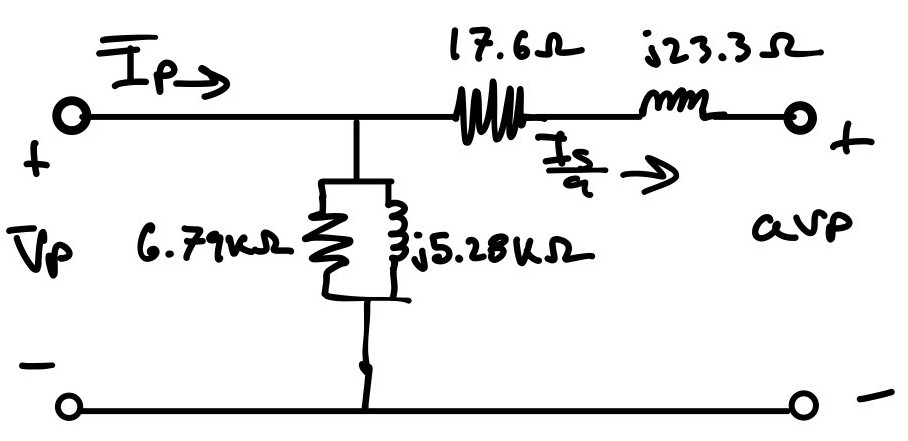
\includegraphics[scale=0.35]{figures/Cantilever eq_1}
	\caption{Cantilever Equivalent Circuit}
\end{figure}